% Variables

% \chapter{Variables and methods to predict the BTC price} % Chapter title

% \label{ch:variables}

%----------------------------------------------------------------------

\chapter{Statistical variable analysis}
\label{ch:stat-var-analysis}

This section describes the basic properties of each feature we are
using in this particular thesis. Among them we have the count of all
variables, mean, standard deviation, min value, max value, quartiles.
We also add the histogram to have an idea of how the distribution of
the variable works and the boxplot that can help us determine if there
are outliers in the data-set.

There are 16 variables descriptions, two of them are sets of
variables, namely, \textit{Bitcoins Days Destroyed}, which groups two
individual variables, and \textit{Standard \& Poors 500}, which groups
another two individual variables. Therefore in the data-set, every
individual member of said sets, would count as an individual feature
for prediction purposes.

The data-sets were obtained from a variaty of sources, but mostly from
\href{https://blockchain.info/charts}{blockchain.info}, excluding
\textit{Euro price in USD} that was obtained from the
\href{https://www.ecb.europa.eu/stats/exchange/eurofxref/html/index.en.html}{European
  Central Bank} web site, and the \textit{Standard \& Poors 500} that
was obtained from
\href{https://finance.yahoo.com/q/hp?s=^GSPC\&a=00\&b=3\&c=1950\&d=05\&e=8\&f=2016\&g=d}{Yahoo!
  Finance}.

While all the data-set have daily data points for their values, they
have different spanning dates, been \textit{Euro price in USD} and
\textit{Standard \& Poors 500} that span the most, because they have
more history than Bitcoin. After analyzing the date span of each
variable, we conclude that the interesction of all the sets is in the
range between 2009-01-03 and 2016-04-28.

\section{Bitcoin Days Destroyed}
\label{sec:bitcoin-days-destroyed}

\textit{Bitcoin Days Destroyed} is a weighted measure of aggregate
economic activity, placing value on transacted coins in proportion to
the time they have spent idle on the Bitcoin blockchain. For any given
transaction, \textit{Bitcoin Days Destroyed} is calculated by
multiplying its estimated transaction value by the number of days
since the coins within the transaction were last spent. It is a useful
proxy for measuring growth in real value transacted on the Bitcoin
blockchain over time, since it controls for rapid movement of coins
between wallets (potentially owned by just one entity). One integer
data point each day, at 18:15:05, spanning from 03/01/2009 to
28/04/2016.

To better understand this variable we include a quote extracted from
\href{http://bitcoin.stackexchange.com/questions/845/what-are-bitcoin-days-destroyed}{Bitcoin
Beta | Stack Exchange}:

``\textit{The idea of "bitcoin days destroyed" came about because it
was realized that total transaction volume per day might be an
inappropriate measure of the level of economic activity in Bitcoin.
After all, someone could be sending the same money back and forth
between their own addresses repeatedly. If you sent the same 50 btc
back and forth 20 times, it would look like 1000 btc worth of
activity, while in fact it represents almost nothing in terms of real
transaction volume.}

\textit{With "bitcoin days destroyed", the idea is instead to give
more weight to coins which haven't been spent in a while. To do this,
you multiply the amount of each transaction by the number of days
since those coins were last spent. So, 1 bitcoin that hasn't been
spent in 100 days (1 bitcoin * 100 days) counts as much as 100
bitcoins that were just spent yesterday (100 bitcoins * 1 day).
Because you can think of these "bitcoin days" as building up over time
until a transaction actually occurs, the actual measure is called
"bitcoin days destroyed". This is believed to give a better indication
of how much real economic activity is occurring on the bitcoin
network.}

\textit{ So how well does it work? Well, it's still not perfect,
because the other day I moved some coins out of a wallet they've been
in for several months without spending them or giving them away. And
some genuine businesses have very rapid turnover in bitcoins, so
they're not being measured well by this method. But it does do a good
job of filtering out the "noise" of bitcoins that are just "bouncing
around" without really going anywhere. The graph of overall bitcoin
days destroyed is believed to show that the genuine level of activity
in the Bitcoin economy is continually increasing--it's not just one
person experimenting by rapidly sending the same coins back and forth,
flooding the network with meaningless chatter. Looks pretty good,
hey?}''

In \autoref{fig:bitcoin-days-destroyed-over-time} we show data over
time for \textit{Bitcoin Days Destroyed}.

\begin{figure}[bth]
  \myfloatalign
  {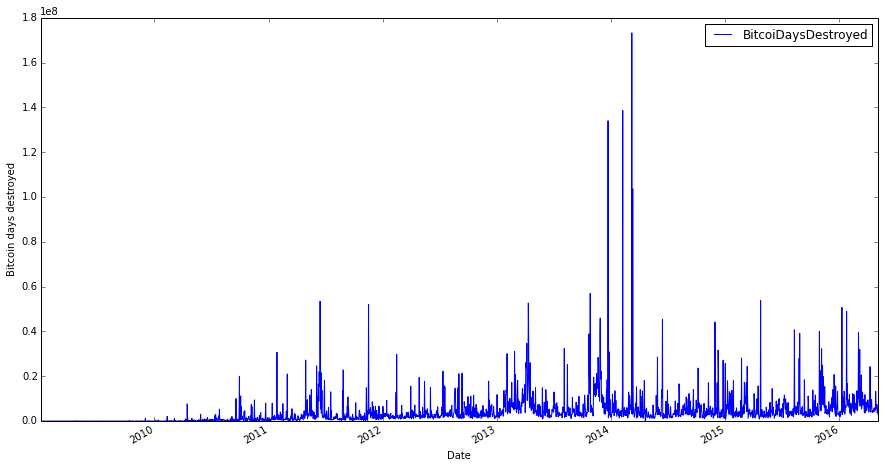
\includegraphics[width=1\linewidth]
    {gfx/bitcoin-days-destroyed-over-time}}
  \caption{\textit{Bitcoin days destroyed} chart}
  \label{fig:bitcoin-days-destroyed-over-time}
\end{figure}


% ----------------------------------------------------------------------

\section{Cost Per Transaction}
\label{sec:cost-per-transaction}

This variable shows miners revenue (in USD) divided by the number of
transactions. Miners revenue are a result of the transaction fees plus
the reward for block discovery. The block discovery reward is fixed by
the community, and is up to the miner to accept any transaction
regardless of the fee in the transaction. A miner can choose not to
add any transaction at all to the block, or add transactions with a
$0$ BTC fee.

\autoref{fig:cost-per-transaction-over-time} shows that in the end of
2010 the Cost Per Transactions started to increase and had a local
maximum followed by another local maximum in mid 2011. This two peaks
took place in a low price of Bitcoin scenario, hence probably the
blocks were introduced with a small amount of transactions, and with a
subtle increase in the Bitcoin price the ratio would increase.

\begin{figure}[bth]
  \myfloatalign
  {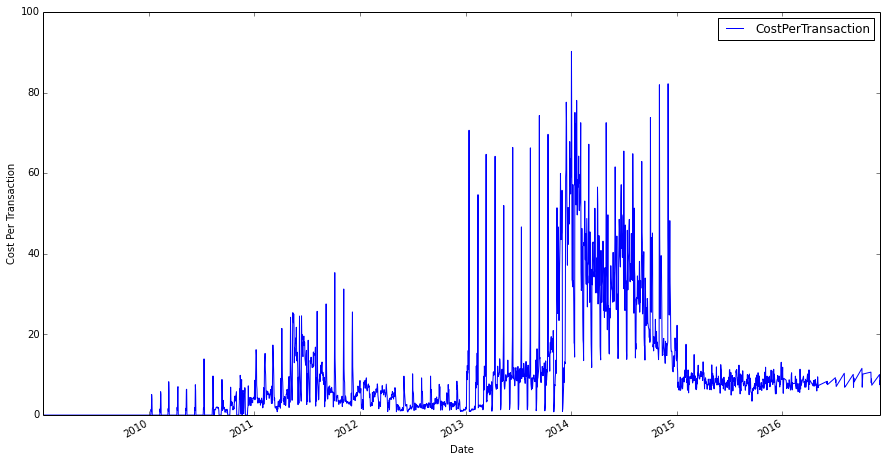
\includegraphics[width=1\linewidth]
    {gfx/cost-per-transaction-over-time}}
  \caption{\textit{Cost per transaction} chart}
  \label{fig:cost-per-transaction-over-time}
\end{figure}

On the contrary, the two peaks of 2014 are in the highest price of the
Bitcoin history, where the number of transactions would make little
effect. Price in that period fluctuates between $700$ USD and $1100$
USD approximately.

\autoref{tab:cost-per-transaction} shows us that the median revenue is
$6.199964$ USD and the mean is $9.731184$ USD. This information is
later increased in \autoref{sec:cost-per-transaction-percent}.

\begin{table}[bth]
  \myfloatalign
  \tiny
  \begin{tabularx}{\textwidth}{XX} 
    \toprule
    \tableheadline{Measure} & \tableheadline{Value} \\
    \midrule
    count  & $2673$      \\
    mean   & $9.731184$  \\
    std    & $13.280920$ \\
    min    & $0$         \\
    $25\%$ & $1.295504$  \\
    $50\%$ & $6.199964$  \\
    $75\%$ & $10.413847$ \\
    max    & $90.202095$ \\
    \bottomrule
  \end{tabularx}
  \caption{Statistical values for \textit{Cost per transaction}}
  \label{tab:cost-per-transaction}
\end{table}

%----------------------------------------------------------------------

\section{Cost Per Transaction Percent}
\label{sec:cost-per-transaction-percent}

This variable shows miners revenue as percentage of the transaction
volume. \autoref{fig:cost-per-transaction-percent-over-time} shows is
that the miners revenue has been near to zero all the time, excluding
few exceptions.

\begin{figure}[bth]
  \myfloatalign
  {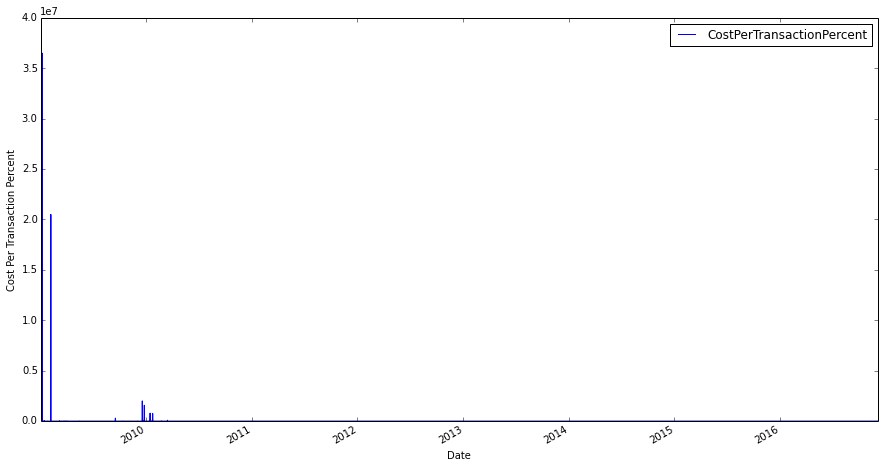
\includegraphics[width=1\linewidth]
    {gfx/cost-per-transaction-percent-over-time}}
  \caption{\textit{Cost per transaction percent} chart}
  \label{fig:cost-per-transaction-percent-over-time}
\end{figure}

As of 2016, miners are more concerned about the reward obtained by
discovering new blocks in the Bitcoin network. In the future the
median percentage is $3.297002$ (see
\autoref{tab:cost-per-transaction-percent}) will probably increase,
because the sole income for miners will be transaction fees.

\begin{table}[bth]
  \myfloatalign
  \tiny
  \begin{tabularx}{\textwidth}{XX} 
    \toprule
    \tableheadline{Measure} & \tableheadline{Value} \\
    \midrule
    count  & $2673$         \\
    mean   & $2.364769e+04$ \\
    std    & $8.113123e+05$ \\
    min    & $0$            \\
    $25\%$ & $1.583523$     \\
    $50\%$ & $3.297002$     \\
    $75\%$ & $9.613778$     \\
    max    & $3.65e+07$     \\
    \bottomrule
  \end{tabularx}
  \caption{Statistical values for \textit{Cost per transaction percent}}
  \label{tab:cost-per-transaction-percent}
\end{table}

%----------------------------------------------------------------------

\section{Estimated Transaction Volume}
\label{sec:estimated-transaction-volume}


The total estimated value of transactions on the Bitcoin blockchain
(does not include coins returned to sender as change). The transaction
volume represented in
\autoref{fig:estimated-transaction-volume-over-time} is very slowly
increasing, meaning that more transactions in Bitcoin are processed.
However, it doesn't represent the actual value of transactions,
because people think in their local currency when trading or shopping,
and Bitcoin's value is volatile. The next variable, \textit{Estimated
  Transaction Volume USD}, is more appropriate for measuring the
transactions volume as it gives us the value of transactions in USD.
The peak that happened in 2012 wouldn't occur easily today due to the
current value of Bitcoin.

\begin{figure}[bth]
  \myfloatalign
  {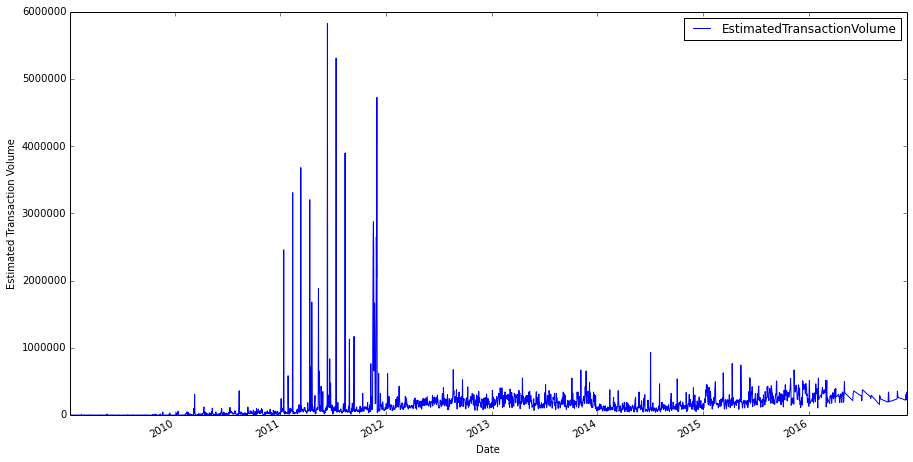
\includegraphics[width=1\linewidth]
    {gfx/estimated-transaction-volume-over-time}}
  \caption{\textit{Estimated transaction volume} chart}
  \label{fig:estimated-transaction-volume-over-time}
\end{figure}

%----------------------------------------------------------------------

% \section{Estimated Transaction Volume USD}
% \label{sec:estimated-transaction-volume-usd}


% The Estimated Transaction Volume in USD value, shown in
% \autoref{fig:estimated-transaction-volume-usd-over-time}, can be
% explained by the average value of Bitcoin, shown in
% \autoref{fig:market-price-over-time}, because nearly all the events
% are paired in the two figures. There is a small increase in estimated
% transaction volume in USD in mid 2011 at the same time than the
% average price of Bitcoin increases. Later on, in 2013 there is a
% bigger increase in estimated volume that is also reflected in the
% average price. Then we have the two biggest peaks around January of
% 2014 coinciding with the highest average value of Bitcoin (also
% represented in two peaks). After that there is decrease in average
% price and estimated volume till 2016 where Bitcoin average price
% starts to increase at the same time that the estimate transaction
% volume increases.

% \begin{figure}[bth]
%   \myfloatalign
%   {\includegraphics[width=1\linewidth]
%     {gfx/estimated-transaction-volume-usd-over-time}}
%   \caption{\textit{Estimated transaction volume USD} chart}
%   \label{fig:estimated-transaction-volume-usd-over-time}
% \end{figure}

% %----------------------------------------------------------------------

\section{Difficulty}
\label{sec:difficulty}


This variable depicts a relative measure of how difficult it is to
find a new block. The \textit{Difficulty} is adjusted periodically as
a function of how much hashing power has been deployed by the network
of miners. \autoref{fig:difficulty-over-time} displays the difficulty
values over time. It can be noticed the staggered nature of the
values, that is because the \textit{Difficulty} is adjusted
automatically every 2016 blocks, and changes equally for the entire
Bitcoin network. Until 2014, the difficulty of mining was very low, it
started to raise probably because the trade volume in the end of 2013
and start of 2014 was approximately 70.000.000\$, which attracted
professional miners with a greater processing power, those creating
more and more blocks and augmenting the difficulty of mining.

\begin{figure}[bth]
  \myfloatalign
  {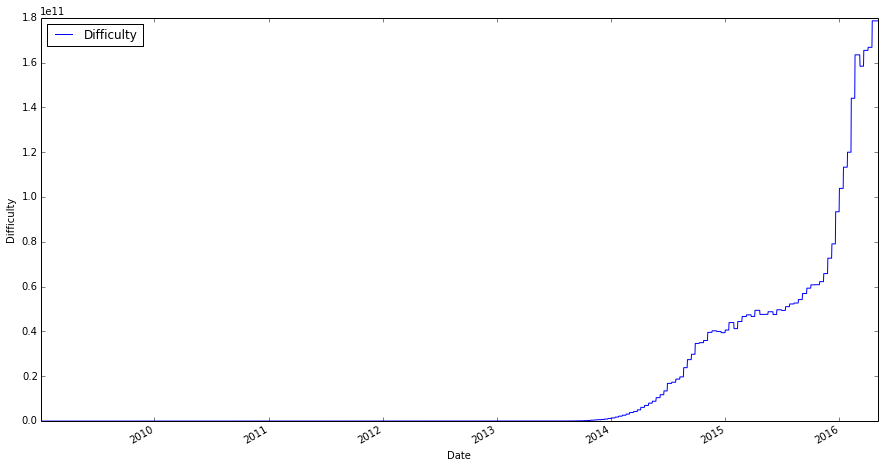
\includegraphics[width=1\linewidth]
    {gfx/difficulty-over-time}}
  \caption{\textit{Difficulty} chart}
  \label{fig:difficulty-over-time}
\end{figure}

%----------------------------------------------------------------------

\section{Euro price in USD}
\label{sec:euro-price-in-usd}


Euro price in USD provided by the European Central Bank from the
creation of the Euro. We have found latent values which have been
interpolated in order to fill the missing values.

As shown in \autoref{fig:euro-price-in-usd-over-time} the value of Euro
has been above that of the USD from its creation, been the period of
2000 through 2003 its closer price to each other. From 2003 to 2007
the price of the Euro increased, coinciding with an increase on the
interest imposed by the BCE. This increase in the interest of the
credits is followed by the collapse of the housing bubble in 2007,
where the price of the Euro kept increasing, altough the interest was
maintained by the BCE until 2009 where the BCE started to lower it.
The increase in the Euro price is probably due to strategies of the
Federal Reserve to lower the price of the USD. Finally in 2015, the
BCE lowered the interests of credits approaching the $0.0\%$, and
that's reflected with a decrease in the price of the Euro with respect
to USD.

\begin{figure}[bth]
  \myfloatalign
  {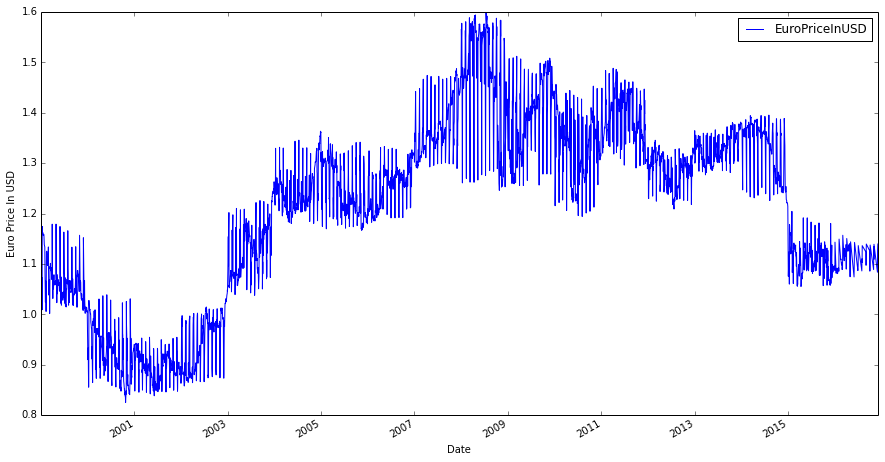
\includegraphics[width=1\linewidth]
    {gfx/euro-price-in-usd-over-time}} 
  \caption{\textit{Euro price in USD} chart}
  \label{fig:euro-price-in-usd-over-time}
\end{figure}

%----------------------------------------------------------------------

\section{Market Price}
\label{sec:market-price}



The USD value of Bitcoin, as calculated by the daily average market
price across major exchanges. This variable is related to many others,
starting with the number of transactions, that can explain the
fluctuations in the Bitcoin price and different events. In March 9,
2011, the Bitcoin reaches parity with USD which is shown in a timid
growth in market price followed by a decrease (see
\autoref{fig:market-price-over-time}).

\begin{figure}[bth]
  \myfloatalign
  {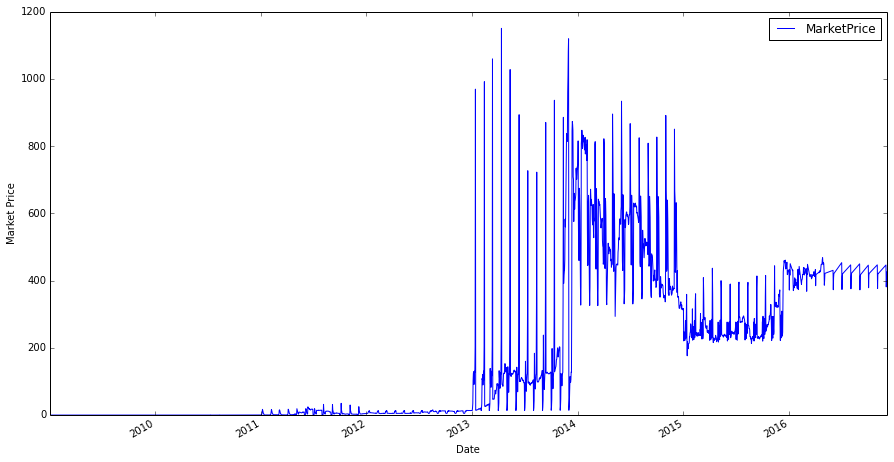
\includegraphics[width=1\linewidth]
    {gfx/market-price-over-time}}
  \caption{\textit{Market price} chart}
  \label{fig:market-price-over-time}
\end{figure}

After that there isn't a big growth until 2013, where several things
happen, Mega, the cloud storage service, starts accepting Bitcoins,
Internet Archive starts accepting Bitcoins, a new food service
\href{PizzaForCoins.com}{PizzaForCoins.com} accepts Bitcoins as a
payment for food, CoinDesk is launched by Spotify investor and
Coinbase receives 5 million USD in funding. This, and several other
events increase the market price of Bitcoin.

After that there is a decrease in market price of Bitcoin, maybe
because MtGox, the largest exchange operator at the time, was seized
by The United States Department of Homeland Security.

In the second half of 2013, various events happen that can be the
cause of the raise of Bitcoin market price, first, in August 6th,
Bitcoin is ruled currency by a Texas judge, then in August 20th,
Bitcoin is ruled as private money in Germany, then in August 28th,
RoboCoin, a Bitcoin ATM manufacturer, starts accepting orders. This
can be the cause of the huge peek at the end of 2013 and start of
2014, where it reaches its highest value (see
\autoref{tab:market-price}). There are no clear events in the Bitcoin
history that explain the period after 2014, which leads us to think
that the price has been fluctuating due to trading strategies.

\begin{table}[bth]
  \myfloatalign
  \tiny
  \begin{tabularx}{\textwidth}{XX} 
    \toprule
    \tableheadline{Measure} & \tableheadline{Value} \\
    \midrule
    count & $2673$ \\
    mean & $155.375541$ \\
    std & $218.398495$ \\
    min & $0$ \\
    $25\%$ & $0.199$ \\
    $50\%$ & $12.28$ \\
    $75\%$ & $270$ \\
    max & $1151$ \\
    \bottomrule
  \end{tabularx}
  \caption{Statistical values for \textit{Market price}}
  \label{tab:market-price}
\end{table}

Is important to note how volatile is the Bitcoin average price,
ranging from nearly $0$ USD to $1151$ USD in just a year (see
\autoref{tab:market-price}), and now, in 2016 fluctuating in a range
bigger than $10$ USD on average. These fluctuations, if predicted, can
be very profitable for the trader.

%----------------------------------------------------------------------

\section{Median Confirmation Time}
\label{sec:median-confirmation-time}

The median time for a transaction to be accepted into a mined block
and added to the public ledger (note: only includes transactions with
miner fees). Until the end of 2011, the confirmation time is
negligible. There is an important event that can be related to the
growth of the median confirmation time, and that is the largest
Bitcoin fee in a single transaction, in December 12, 171 Bitcoins was
paids as fee in block 157235.

If we look at \autoref{fig:median-confirmation-time-over-time} there
is a peak in mid 2012, that can coincide with the increase in
\textit{Output Volume} seen in \autoref{fig:output-volume-over-time}.

\begin{figure}[bth]
  \myfloatalign
  {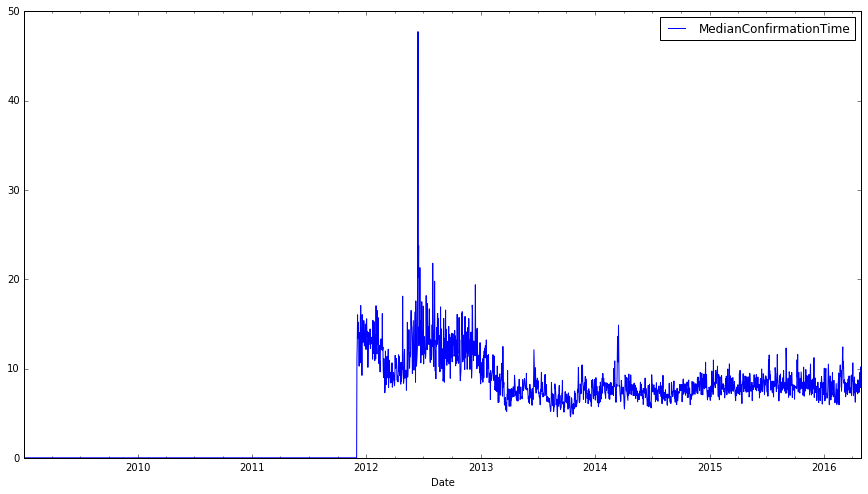
\includegraphics[width=1\linewidth]
    {gfx/median-confirmation-time-over-time}}
  \caption{\textit{Median confirmation time} chart}
  \label{fig:median-confirmation-time-over-time}
\end{figure}

% ----------------------------------------------------------------------

\section{Number of Transactions}
\label{sec:n-transactions-multiple}

Here we analyze \textit{Number of transactions}, which is defined as
``\textit{The number of daily confirmed Bitcoin transactions}''. The
\textit{Number of transactions} represented in
\autoref{fig:n-transactions-over-time} show a moderated
growth compared to that of the market price. That may be because this
variable doesn't depend on the inflation of the Bitcoin, and there
aren't exagerated fluctuation. We see that even the price of the
Bitcoin is not at its peak in 2016, the \textit{Number of
  transactions} are at its higher point so far in the Bitcoin history.

\begin{figure}[bth]
  \myfloatalign
  {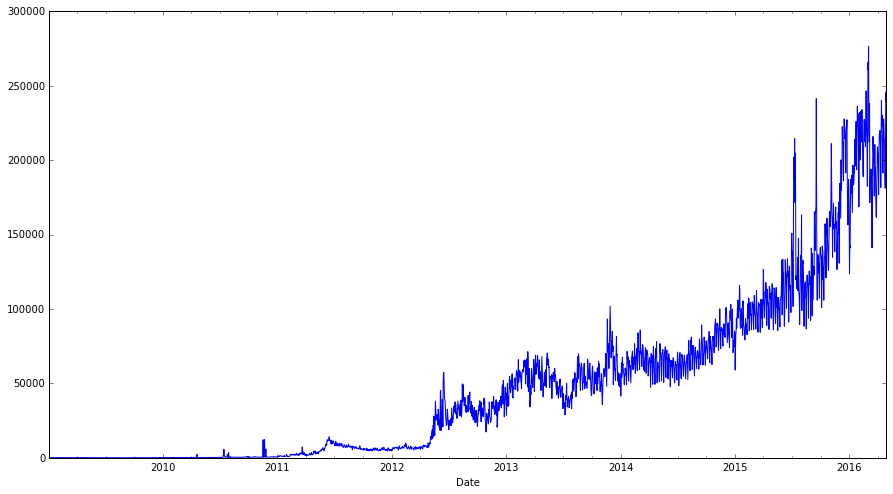
\includegraphics[width=1\linewidth]
    {gfx/n-transactions-over-time}}
  \caption{\textit{Number of transactions} chart}
  \label{fig:n-transactions-over-time}
\end{figure}

% ----------------------------------------------------------------------

\section{Output Volume}
\label{sec:output-volume}

The total value of all transaction outputs per day (includes coins
returned to the sender as change). There are a lot of events that
appear in \textit{OutputVolume}(\autoref{fig:output-volume-over-time})
that also appear in
\textit{MarketPrice}(\autoref{fig:market-price-over-time}) showing
that there is a strong relationship between the two measures.

\begin{figure}[bth]
  \myfloatalign
  {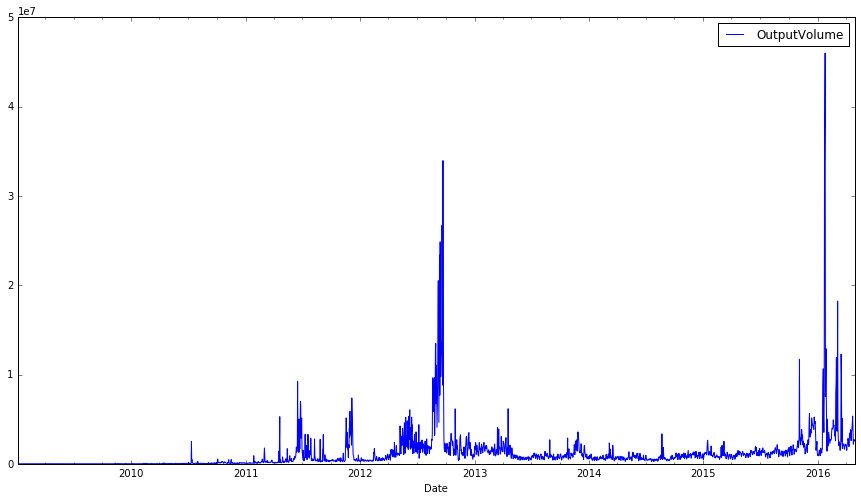
\includegraphics[width=1\linewidth]
    {gfx/output-volume-over-time}}
  \caption{\textit{Output volume} chart}
  \label{fig:output-volume-over-time}
\end{figure}

It's easier to understand the meaning of output and change returned to
the sender in the Bitcoin world with an explanation given by a user
nicknamed \textit{DeathAndTaxes} in
\href{https://bitcointalk.org/index.php?topic=99593.0}{Bitcointalk.org}:

``\textit{Bitcoin can only create transactions by using as the input
  an ENTIRE prior unspent output. The most important thing to realize
  is that Bitcoin tx have inputs and outputs. The "value" of your
  wallet is an abstraction. It is simply your client (software which
  analyzes the wallet) taking a SUM of all the unspent outputs which
  you have private keys for. The input of a tx is the output of a
  PRIOR tx. You can only use unspent outputs in a new tx. Once they
  are part of a tx they can never be used again ("spent").}

\textit{Say you I send you 50 BTC (for simplicity lets assume this is
  compromised of a single 50 BTC output). No matter how you spend that
  the input for the tx will be 50 BTC.}

\textit{Want to spend 20 BTC? Input: 50 BTC Output: 20 BTC + 30 BTC
  "change" back to an address you control. Want to spend 1 BTC? Input:
  50 BTC Output: 1 BTC + 49 BTC "change" back to an address you
  control.}''

Output can be due to three circumstances, large amout of transactions,
transactions of big amount of Bitcoins, and big amount of change
returned to sender. The peak of 2013 is clearly due to change received
by sender as \textit{DeathAndTaxes} explains: ``\textit{In the early
  days of Bitcoin there really was nothing to "spend" it on so most tx
  tended to be accumulation. This resulted in most addresses having
  very large unspent outputs. As people started "breaking" up those
  unspent outputs in tx involving smaller amounts most of the volume
  WAS change.}''

%--------------------------------------------------------------------- 

\section{Standard \& Poors 500}
\label{sec:standard-and-poors-500}


From the
\href{https://en.wikipedia.org/wiki/S\%26P_500_Index}{Wikipedia}:

``\textit{The Standard \& Poor's 500, often abbreviated as the S\&P
  500, or just "the S\&P", is an American stock market index based on
  the market capitalizations of 500 large companies having common
  stock listed on the NYSE or NASDAQ. The S\&P 500 index components
  and their weightings are determined by S\&P Dow Jones Indices. It
  differs from other U.S. stock market indices, such as the Dow Jones
  Industrial Average or the Nasdaq Composite index, because of its
  diverse constituency and weighting methodology. It is one of the
  most commonly followed equity indices, and many consider it one of
  the best representations of the U.S. stock market, and a bellwether
  for the U.S. economy. The National Bureau of Economic Research has
  classified common stocks as a leading indicator of business
  cycles.}''

We can see the description of certain events of
\autoref{fig:standard-and-poors-500-over-time} also from
\href{https://en.wikipedia.org/wiki/S\%26P_500_Index}{Wikipedia}:

\begin{figure}[bth]
  \myfloatalign
  {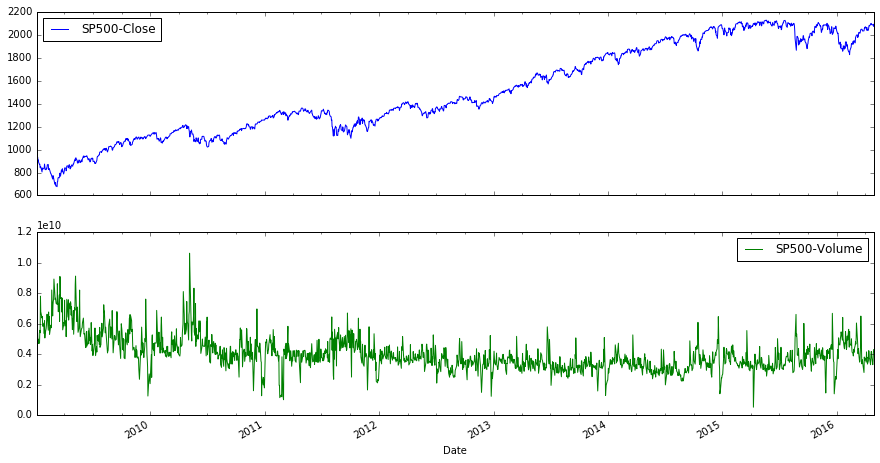
\includegraphics[width=1\linewidth]
    {gfx/standard-and-poors-500-over-time}}
  \caption{\textit{Standard \& poors 500}
    chart}
  \label{fig:standard-and-poors-500-over-time}
\end{figure}

``\textit{In mid-2007, the subprime mortgage crisis spread to the wider
  U.S. financial sector. The resulting situation became acute in
  September 2008, ushering in a period of unusual market volatility,
  encompassing record 100-point swings in both directions and reaching
  the highest levels since 1929. On November 20, 2008, the index
  closed at 752.44, its lowest since early 1997. A modest recovery the
  following day still left the index down 45.5\% for the year. This
  year-to-date loss was the greatest since 1931, when the broad market
  declined more than 50\%. The index closed the year at 903.25, for a
  loss of 38.5\%. The market continued to decline in early 2009,
  surrounding the financial crisis of 2008. The index reached a nearly
  13-year low, closing at 676.53, on March 9, 2009.}

\textit{On March 23, 2009, the S\&P 500 marked a 20\% gain when it hit
  822.92. The Dow Jones Industrial Average soon followed. The close
  for 2009 was 1,115.10, making it the second-best year of the decade.
  On April 14, 2010 the index broke 1200 closing at 1210.65, but by
  July 2, 2010 it had closed at 1022.58. On April 29, 2011, the index
  closed at 1363.61, but it had a sharp drop in August and briefly
  broke 1100 in October (with the VIX hitting 40). Gains continued
  despite significant volatility amid electoral and fiscal
  uncertainty, and the 2012 close of the S\&P 500 following QE3 was
  its third-highest ever, at 1,426.22 points. Many people hated the
  bull market. On March 28, 2013, it closed above the closing high
  from 2007. On April 10, 2013, it also closed above the intraday high
  from 2007.}

\textit{On May 3, 2013—more than 13 years since its first close above
  1,500—the S\&P 500 closed above 1,600 for the first time, at
  1,614.42. This would be the first of three 100-point milestones in
  2013: 1,600 on May 3, 2013; 1,700 on August 1, 2013; and 1,800 on
  November 22, 2013. The S\&P 500 closed out 2013 at a record high,
  finishing the December 31, 2013, trading day at 1,848.36. On May 23,
  2014, the index for the first time closed above 1,900, at 1,900.53.
  On August 26, 2014, the index closed above 2,000 for the very first
  time, and on December 22 the S\&P 500 climbed to 2078, an all-time
  high. The index closed on December 29 at 2,090.57 with a closing of
  2,058.90 at the end of 2014. This was a gain of 85\% (in price
  return, and 105\% in total return) for the five years 2010-2014. On
  February 17, 2015, the index first closed above 2,100, closing at
  2,100.34. On February 25, 2015 it reached 2,119.59 during mid-day,
  and on the following day it closed at record high of 2,115.48. On
  May 21, 2015, the index closed at 2,130.82, its high point for the
  year. At the close of 2015, the index hit 2,043.94, down 0.73\% for
  the year.}''

Variable \textit{Close} has a linear increasing trend which can
probably be explained because of the inflation, while the volume is a
random walk, following no apparent trend or seasonality. To complete
the information and better understand the graphics shown the reader
can analyze \autoref{tab:standard-and-poors-500}.

\begin{table}[bth]
  \myfloatalign
  \tiny
  \begin{tabularx}{\textwidth}{XXX} 
    \toprule
    \tableheadline{Measure} & \tableheadline{SP500-Close}
    & \tableheadline{SP500-Volume} \\
    \midrule
    count  & $2673$        & $2673$    \\
    mean   & $1503.979515$ & $4.000942e+09$ \\
    std    & $395.164083$  & $1.122921e+09$ \\
    min    & $676.530029$  & $5.362e+08$    \\
    $25\%$ & $1178.339966$ & $3.299395e+09$ \\
    $50\%$ & $1406.290039$ & $3.78247e+09$  \\
    $75\%$ & $1898.293335$ & $4.50811e+09$  \\
    max    & $2130.820068$ & $1.061781e+10$ \\
    \bottomrule
  \end{tabularx}
  \caption{Statistical values for \textit{Standard \& poors 500}}
  \label{tab:standard-and-poors-500}
\end{table}

% ---------------------------------------------------------------------

\section{Total Bitcoins}
\label{sec:total-bitcoins}

The total number of bitcoins that have already been mined; in other
words, the current supply of bitcoins on the network. First we have to
know that, according to the \href{}{Wikipedia} ``The bitcoin protocol
specifies that the reward for adding a block will be halved every
210000 blocks (approximately every four years). Eventually, the reward
will decrease to zero, and the limit of 21 million bitcoins will be
reached circa 2140; the record keeping will then be rewarded by
transaction fees solely.'' As shown in
\autoref{fig:total-bitcoins-over-time} the growth of bitcoin amount
will decrease every time the difficulty increases, with 21 million
been the upper limit. This change in difficulty depend on the blocks
discovered by miners.

\begin{figure}[bth]
  \myfloatalign
  {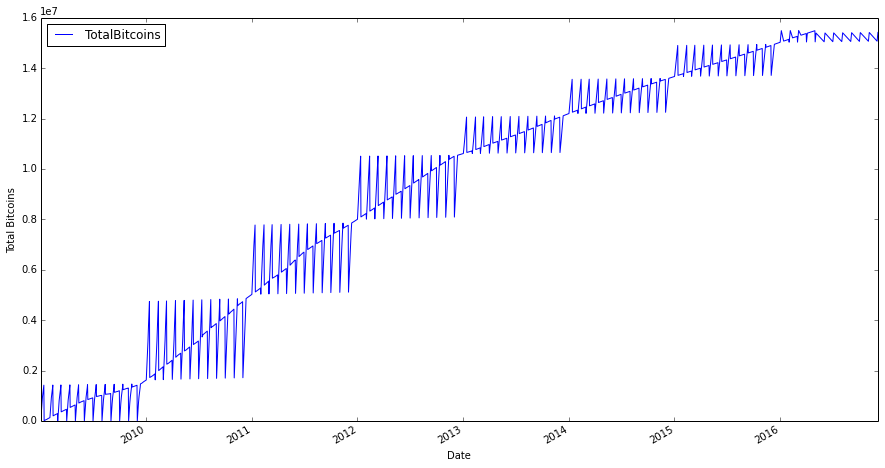
\includegraphics[width=1\linewidth]
    {gfx/total-bitcoins-over-time}}
  \caption{\textit{Total bitcoins} chart}
  \label{fig:total-bitcoins-over-time}
\end{figure}

%--------------------------------------------------------------------- 

\section{Trade Volume}
\label{sec:trade-volume}

The total USD value of trading volume on major Bitcoin exchanges.

By comparing
\textit{TradeVolume}(\autoref{fig:trade-volume-over-time}) with other
figures as \textit{MarketPrice}(\autoref{fig:market-price-over-time})
it's clear that there is a big bound between trade volume and market
price of Bitcoin. There are peaks in mid 2011, March of 2013, December
of 2013, and the end of 2015 in both variable, showing the
aforementioned relationship.

\begin{figure}[bth]
  \myfloatalign
  {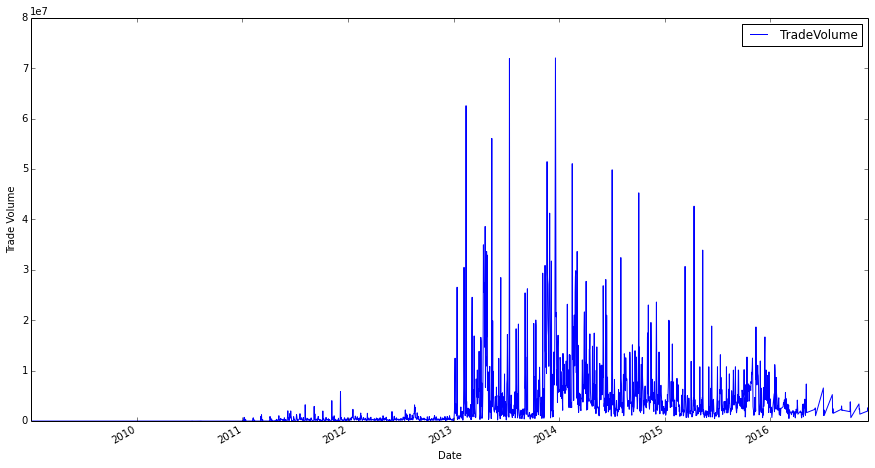
\includegraphics[width=1\linewidth]
    {gfx/trade-volume-over-time}}
  \caption{\textit{Trade volume}
    chart}
  \label{fig:trade-volume-over-time}
\end{figure}

Trade volume doesn't really exhibit the real activity in the Bitcoin
network, because with this variable we don't see the transactions
between users. There is also another pattern that can be seen in the
trade volume, is that when the market price is maintained the trade
volume decreases, meaning that people are interested in the Bitcoin
exchange when its price fluctuates.

%--------------------------------------------------------------------- 

\section{Transaction Fees}
\label{sec:transaction-fees}

The total value of all transaction fees paid to miners (not including
the coinbase value of block rewards) in BTC. This variable depends on
the amount of transactions and the amount of fee paid per transaction.
If we look at
\textit{TransactionsFees}(\autoref{fig:transaction-fees-over-time}) we
can see that even there is an increase in the number of transactions
near the peaks, the height of those peaks is not comparable, in
consequence we can assume that at least those peaks are not due
entirely to the number of transactions made. We can see that there is
some relationship with
\textit{MarketPrice}(\autoref{fig:market-price-over-time}), reflecting
how ``\textit{eager}'' is the user to have the transaction accepted.
This relationship is not in the sense that the peaks appear
simultaneously in the charts, but the peaks of
\textit{TransactionFees} procede those of \textit{MarketPrice}. This
can also be due to the low price of Bitcoin in those
\textit{TransactionFees} peaks, because people think in USD mostly, so
they fix the price of the fee in USD instead of BTC producing those
rises.

\begin{figure}[bth]
  \myfloatalign
  {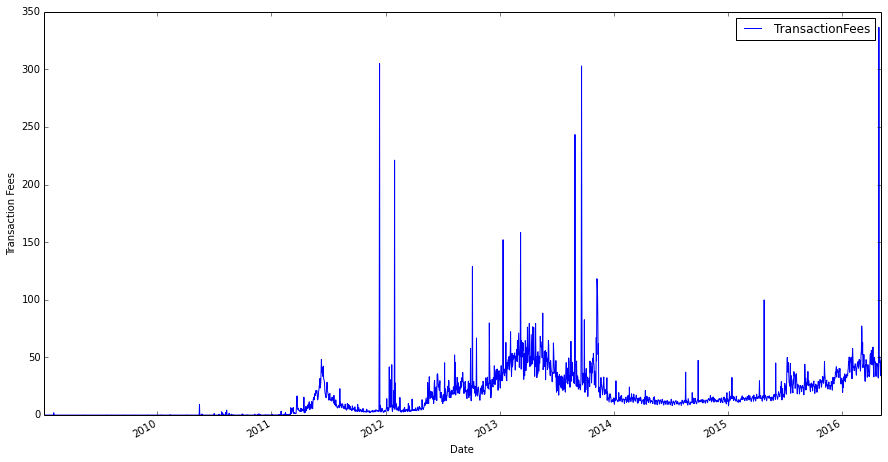
\includegraphics[width=1\linewidth]
    {gfx/transaction-fees-over-time}}
  \caption{\textit{Transaction Fees} chart}
  \label{fig:transaction-fees-over-time}
\end{figure}

%--------------------------------------------------------------------- 

\section{Transaction Fees USD}
\label{sec:transaction-fees-usd}

The total value of all transaction fees paid to miners (not including
the coinbase value of block rewards) in USD.
\textit{TransactionFeesUSD}
(\autoref{fig:transaction-fees-usd-over-time}) shows how the fees
measured in USD are more stable in time than fees measured in BTC
shown in
\textit{TransactionFees}(\autoref{fig:transaction-fees-over-time}).

\begin{figure}[bth]
  \myfloatalign
  {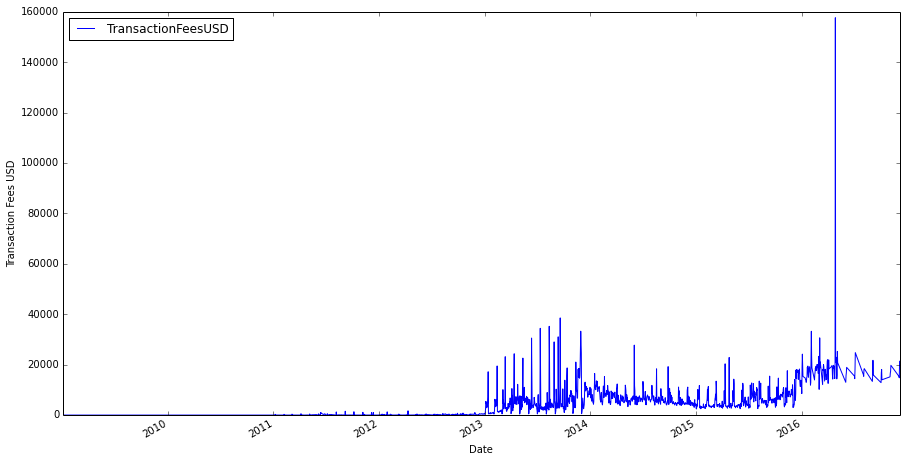
\includegraphics[width=1\linewidth]
    {gfx/transaction-fees-usd-over-time}}
  \caption{\textit{Transaction fees USD} chart}
  \label{fig:transaction-fees-usd-over-time}
\end{figure}

There highest fees prices have been paid in the last half of 2013 and
start of 2014, falling together with the highest price of Bitcoin,
this can be explained because the users would want their transactions
to be processed before others. There is another peak, very localized
because it's only one day where the transactions fees reach
$157676.252$ USD (see \autoref{tab:transaction-fees-usd}), this can be
because the transactions/trade volume ratio is at its highest point
since 2011, which means that Bitcoin transaction volume is even higher
than January of 2014 when the price of Bitcoin was approaching three
times the current price, so we can assume that the Bitcoin transaction
volume is due to number of transactions more than amount of Bitcoin
per transaction.


\begin{table}[bth]
  \myfloatalign
  \tiny
  \begin{tabularx}{\textwidth}{XX} 
    \toprule
    \tableheadline{Measure} & \tableheadline{Value} \\
    \midrule
    count & $2673$ \\
    mean & $3476.856463$ \\
    std & $5990.380532$ \\
    min & $0$ \\
    $25\%$ & $0.001244$ \\
    $50\%$ & $273.841916$ \\
    $75\%$ & $5344.867164$ \\
    max & $157676.252853$ \\
    \bottomrule
  \end{tabularx}
  \caption{Statistical values for \textit{Transaction fees USD}}
  \label{tab:transaction-fees-usd}
\end{table}

%--------------------------------------------------------------------- 

\section{Transactions/Trade Ratio}
\label{sec:tx-trade-ratio}

\textit{TxTradeRatio} (\autoref{fig:tx-trade-ratio-over-time})
presents the relationship between BTC transaction volume and USD
exchange volume. This is another chart that can gives us an idea of
the transactions inside the Bitcoin network, excluding the trading.

\begin{figure}[bth]
  \myfloatalign
  {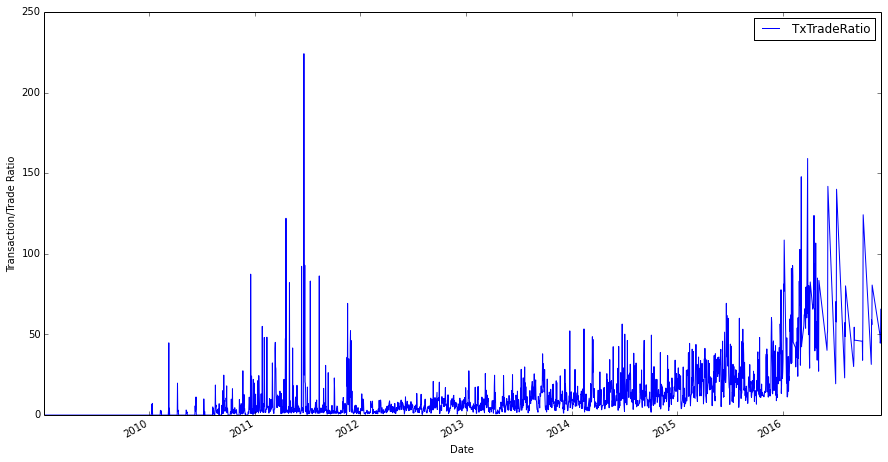
\includegraphics[width=1\linewidth]
    {gfx/tx-trade-ratio-over-time}}
  \caption{\textit{Transactions/trade ratio} chart}
  \label{fig:tx-trade-ratio-over-time}
\end{figure}


High values of this variable can mean two different things. One is
that the value of Bitcoin is very low, as in 2011, and the
transactions between users, no matter how high they are, measured in
Bitcoin, are going to have low values measured in USD. The other
explanation is that there are a lot of transactions inside the Bitcoin
network compared with the USD echange volume, even if the Bitcoin
price is high, which would probably mean that there is a high usage of
Bitcoin as a currency between individuals, this may be the cause of
the raise of this ratio since the end of 2015.

%--------------------------------------------------------------------- 

\section{Wikipedia Trend for Bitcoin}
\label{sec:wikipedia-trend-for-bitcoin}

The particular trend used in this case is the page views per day of
the Bitcoin article in the English version of Wikipedia. The daily
visits to this paige has been as high as $923659$ (see
\autoref{tab:wikipedia-trend-for-bitcoin}), and a mean of
$8168.301160$.

\begin{table}[bth]
  \myfloatalign
  \tiny
  \begin{tabularx}{\textwidth}{XX} 
    \toprule
    \tableheadline{Measure} & \tableheadline{Value} \\
    \midrule
    count & $2673$ \\
    mean & $8168.301160$ \\
    std & $25977.892265$ \\
    min & $0$ \\
    $25\%$ & $86$ \\
    $50\%$ & $4173$ \\
    $75\%$ & $8585$ \\
    max & $923659$ \\
    \bottomrule
  \end{tabularx}
  \caption{Statistical values for \textit{Wikipedia trend for bitcoin}}
  \label{tab:wikipedia-trend-for-bitcoin}
\end{table}

For a better understanding of this variable we can rely on the
ubiquitous \textit{MarketPrice} since Bitcoins allure is it's price
and fluctuation with respect to more stable currencies like USD or
EUR. There are a number of events that can produce the spike produced
in second half of 2015 (see
\autoref{fig:wikipedia-trend-for-bitcoin-over-time}).

\begin{figure}[bth]
  \myfloatalign
  {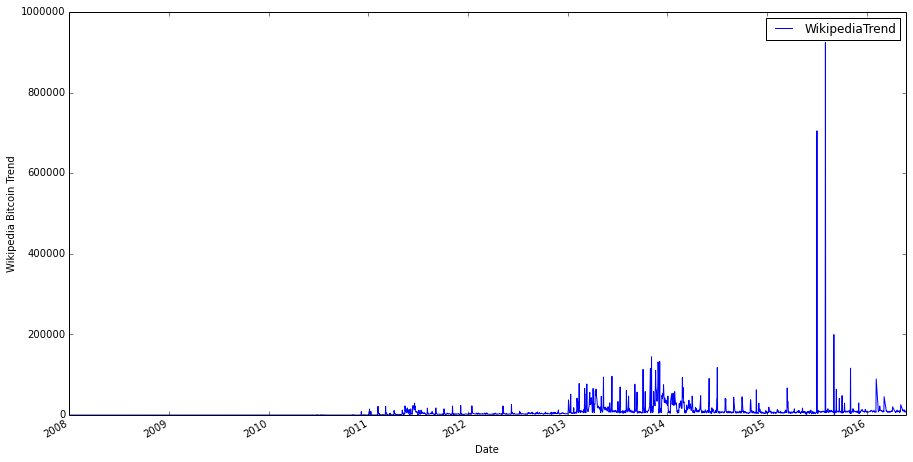
\includegraphics[width=1\linewidth]
    {gfx/wikipedia-trend-for-bitcoin-over-time}}
  \caption{\textit{Wikipedia trend for bitcoin}
    chart}
  \label{fig:wikipedia-trend-for-bitcoin-over-time}
\end{figure}

In January the \textit{New York Stock Exchange} invests $75M$ USD in
Coinbase. In March the results of the UK Treasury's call for
information on digital currency are announced. In May the 19th Ross
Ulbricht, operator of the \textit{Silk Road} marketplace, is sentenced
to life in prison. In June the 3rd, New York state releases the
BitLicense, a set of customized rules meant to regulate Bitcoin and
digital currency businesses that serve customers located in New York
state. In July the 1st, two federal agents plead guilty to Silk Road
theft during their active investigation of the marketplace. In August
the 1st, Mark Karpeles, the CEO of the failed Bitcoin exchange Mt.
Gox, was arrested in Japan on charges of fraud and embezzlement in
relation to collapse of the exchange. Bitcoin Core developers Mike
Hearn and Gavin Andresen released a separate version of the Bitcoin
client software, called Bitcoin XT. The release illustrates an ongoing
controversy in the Bitcoin development community: \textit{What limit
  should be placed on the size of Bitcoin's blocks?}. In October the
22nd, The European Court of Justice ruled that the exchange of Bitcoin
and "virtual currencies" is not subject to value-added-tax (VAT) in
the European Union. In October, the 31st, Bitcoin is featured on front
page of The Economist. In November, the 3rd, Bitcoin sign is accepted
into Unicode. This are all events that may have produced many visits
to the Bitcoin Wikipedia page.

%--------------------------------------------------------------------- 

\chapter{Feature subset selection}
\label{ch:feature-selection}

The process of \textit{feature subset selection (FSS)} used in this
thesis is composed of two steps. One where we choose a set of
variables with \textit{principal component analysis (PCA)}
(\cite{pearson1901liii}) which is going to be our feature super-set
for all the models. Later on, for selecting per-model subsets a
\textit{Wrapper FSS (WFSS)} technique (\cite{kohavi1997wrappers}) is used.

This approach to \textit{FSS} has been taken because wrapper methods
select the best features (\cite{inza2004filter, kumari2011filter})
and, at the same time, they are more computationally expensive than
filter methods. We came out with the mixed approach of selecting a
super-set with \textit{PCA}, which is computationally cheap and then
we selected the final subsets with a wrapper method.

\textit{WFSS} is a greedy algorithm, also called a forward
feature selection. In each iteration a model is produced with a subset
which initially is composed of one variable. In each iteration of the
algorithm the variable that minimizes the error produced is added to
selected features. If in a iteration a variable selected doesn't
minimize the error of the selected features the algorithm has
finished.

The features presented in \autoref{ch:stat-var-analysis} where
obtained by running a \textit{PCA} over 41 variables selecting the 18
that added more information to the prediction.

We can see in \autoref{fig:explained-variance} an ordered
representation of the \textit{Explained variance} of the dimensions
obtained by performing \textit{PCA} over the original data-set. This
information is what led us to choose 17 as the dimensions that has
some meaningful information to predict the \textit{Bitcoin} price.

\begin{figure}[bth]
  \myfloatalign
  {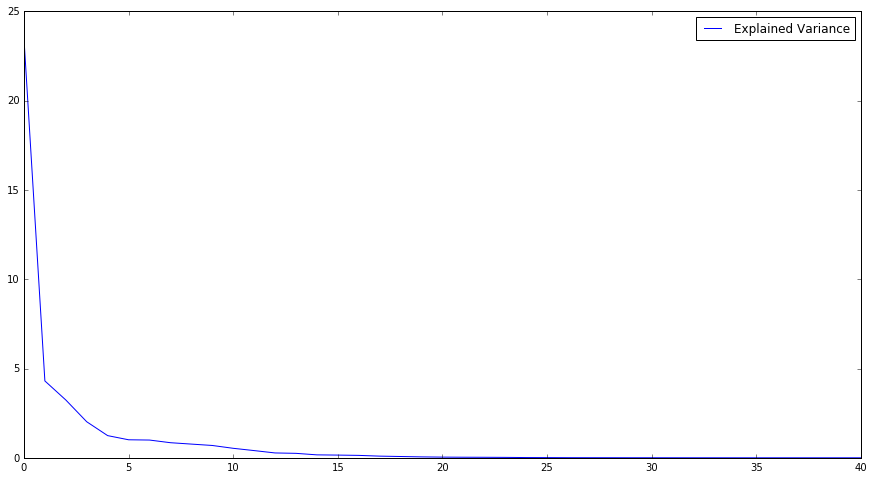
\includegraphics[width=1\linewidth]
    {gfx/explained-variance}}
  \caption{\textit{Explained variance} of PCA dimensions.}
  \label{fig:explained-variance}
\end{figure}

The results of \textit{WFSS} and the parameters used are explained in
\autoref{part:experiment}.

%\enlargethispage{2cm}

%------------------------------------------------

%%% Local Variables:
%%% mode: latex
%%% TeX-master: "../main"
%%% End:
